\documentclass[handout]{beamer}
\usepackage[portuguese]{babel}


\usetheme{Frankfurt}
%\usetheme{Warsaw}
\graphicspath{{figures/}}

\title{Real-time Ethernet Networks: a practical approach to network cycle time influence in control applications}
\author[Sim\~{a}o Amorim \and Paulo Portugal]{Sim\~{a}o Amorim\inst{1} \\ Orientador: Paulo Portugal\inst{1}}
\titlegraphic{\includegraphics[width=2.5cm]{uporto-feup.pdf}}
\institute[Feup]{\inst{1}Departamento de Engenharia Eletrotécnica e de Computadores\\
	Faculdade de Engenharia da Universidade do Porto\\
	EEC0020 - Dissertaç\~{a}o}
\date{8 de outubro de 2021}

\addtobeamertemplate{navigation symbols}{}{%
	\usebeamerfont{footline}%
	\usebeamercolor[fg]{footline}%
	\hspace{1em}%
	\insertframenumber
}

\begin{document}
	\maketitle
	
	\Large
	
	\begin{frame}
	\frametitle{Conte\'{u}do}
	\begin{itemize}
		\item Contexto e motivaç\~{a}o
		\item Objetivos
		\item Revis\~{a}o bibliogr\'{a}fica
		\item Arquitetura do sistema
		\item Resultados experimentais
		\item Conclus\~{o}es
	\end{itemize}
\end{frame}
	
	\section{Context} \label{sec:context}
% * Field network

Modern process control systems include advanced features which were virtually impossible to implement even two decades ago. For many years now, industrial processes have been managed by specialized control hardware such as \textbf Programmable \textbf Logic \textbf Controllers ({\bfseries PLC}).

In the early days, PLCs were very limited in terms of performance and \textbf Input/\textbf Output (I/O) count, so when a process to be controlled was too complex, dividing it into simpler parts was needed. This way, a single complex process was automated by independently automating different parts of it. This was done by giving each part its own dedicated controller and then creating some sort of communication between them, therefore creating a \textbf Distributed \textbf Control \textbf System ({\bfseries\itshape DCS}). Because these controllers were very simple, such communication had to be limited to just a couple of I/O signals between PLC's or very limited digital communication channels like RS-232 \cite{protocol:rs232}. This created a major chokepoint on the amount of information that could be shared between controllers within the same process, ultimately posing hard obstacles to development and troubleshooting of such systems. If somehow these controllers could share more information, not only development and troubleshooting would be easier, but it would also make these complex control systems more adaptable, allowing the development of even more complex automation systems.

%TODO
(Still want to clarify the term \emph{field device}, so I need to talk a bit more about \emph{DCS}s)

With the emergence of digital communication networks, some businesses started to look into ways to bring their power into the industrial automation world. Such networks, as they were, provided far more information throughput than the legacy I/O signals but at the cost of reliability. Automated industrial processes are, a lot of times, critical systems and these need a reliable and deterministic control. Although simple, the legacy I/O signals provided a reliable and deterministic communication channel, but digital networks such as \emph{Ethernet} \cite{protocol:ethernet} do not, especially when it is comprised of more than two devices. As such, in order to reliably replace the communication mechanisms in industrial environments, modifications needed to be made. In the last thirty years, several adaptations of the standardized \emph{Ethernet} protocol have emerged, such as \emph{Ethernet/IP} (2001) \cite{protocol:ethernetip}, \emph{EtherCAT} (2003) \cite{protocol:ethercat} or \emph{PROFINET} (2003) \cite{protocol:profinet}.

The technology advancements in both hardware and software fields have allowed industrial \emph{DCS}s to grow in usage. Modern control systems implementation typically follow the ISA95 \cite{standard:isa95} standard.

%TODO
(Present a ISA95 standard graph)

%TODO
(explain that with the technology advancements, more advanced control is being done with \emph{DCS}s, namely movement control, and that it implies even stricter requirements in terms of communications, meaning that, the deterministic requirement for the network data transmission now means real-time requirement, which comprises low latency and faster response times, AKA, shorter network cycle time)

%TODO
(maybe also talk about Industry 4.0 and the current needs to have every electronic device accessible over a network?)

	\begin{frame}
	\frametitle{Motivaç\~{a}o}
	\begin{itemize}
		\item Nova cadeira sobre redes de comunicaç\~{a}o industriais de tempo-real no MEEC/FEUP;
		\item Proporcionar aos estudantes uma plataforma onde estes possam ter contacto com a tecnologia em quest\~{a}o.
	\end{itemize}
\end{frame}

	\section{Objectives} \label{sec:objectives}
% * solid foundation for future works
% ** hardware accessibility
% ** hardware interchangeability
% ** software modularity
% ** solid documentation
% * network cycle time demonstrator
% ** local control
% ** remote control
% ** position control
% ** velocity control

This thesis mainly intends to produce a solid foundation for practical demonstrators of industrial real-time networks. The work developed on this dissertation will build upon the concept of network cycle time, providing whoever interacts with the proposed solution a practical and reality-based experiment to observe the effects of network cycle time in control application. Because we intend to create a good foundation for different and more advanced demonstrators to be built upon, we aim at providing a robust and well documented solution with a high level of reusability.

In order to provide a network cycle time demonstrator, we will develop a networked \emph{field device} capable of running in two configurations:

\begin{itemize}
	\item Local control: the control loop will be closed on the \emph{field device} itself by means of a simple and fast algorithm which receives the control set-points from the real-time network.
	\item Remote control: the \emph{field device} will work as a simple remote I/O card which will synchronise the physical inputs and outputs with values being transmitted on the real-time network. This will effectively mean the control loop will only be closed on the \emph{process control} device, having the real-time network operate inside this control loop.
\end{itemize}

These configurations allow the user to create a base dataset from the local control configuration and compare the dataset generated by the remote control configuration with that base.
	
	\begin{frame}{Revis\~{a}o Bibliogr\'{a}fica - Aplicações de tempo-real}
	A validade dos dados depende de quando estes foram adquir\'{i}dos
	
	\medskip
	Podem ser classificadas como:
	\begin{itemize}
		\item Hard real-time
		\item Soft real-time
	\end{itemize}
\end{frame}
	\begin{frame}{Revis\~{a}o Bibliogr\'{a}fica - Redes Ethernet de tempo-real}
	Classificadas em tr\^{e}s categorias, de acordo com a abordagem adotada:
	\begin{itemize}
		\item \emph{Top of TCP/IP} % Nenhuma alterç\~{a}o feita aos protocolos de comunicaç\~{a}o, funciona de forma transparente;
		\item \emph{Top of Ethernet} % Pilha protocolar própria a funcionar com base na tecnologia Ethernet, sem lhe aplicar modificações;
		\item \emph{Modified Ethernet} % Pilha protocolar própria a funcionar com base na tecnologia Ethernet mas com modificações no protocolo ou no \emph{hardware}.
	\end{itemize}
\end{frame}
	\begin{frame}{Revis\~{a}o Bibliogr\'{a}fica - EtherCAT}
	Princ\'{i}pio de funcionamento:
	
	\begin{itemize}
		\item 
	\end{itemize}
\end{frame}
	
	\begin{frame}{Arquitetura do Sistema}
	\begin{figure}
		\centering
		\includegraphics[width=0.8\linewidth]{overall-architecture.pdf}
	\end{figure}
\end{frame}
	\begin{frame}{Arquitetura do Sistema - Dispositivo \emph{Slave}}
	\begin{figure}
		\centering
		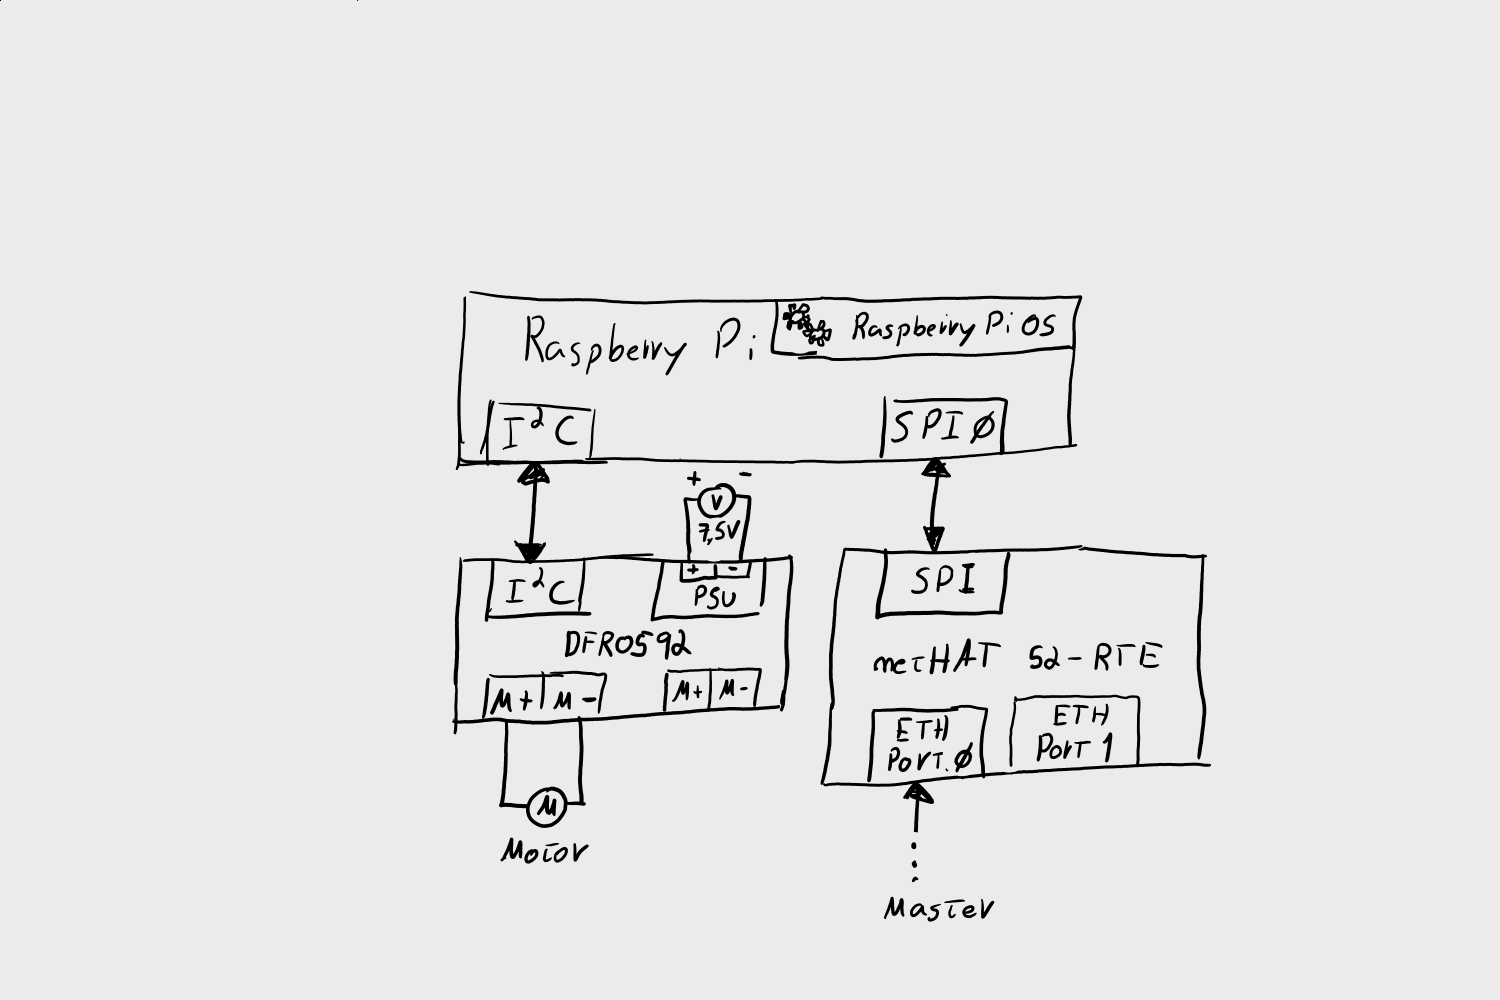
\includegraphics[width=0.8\linewidth]{slave_architecture.pdf}
	\end{figure}
\end{frame}
	\begin{frame}{Arquitetura do Sistema - Dispositivo \emph{Slave}}
	\begin{figure}
		\centering
		\includegraphics[width=0.75\linewidth]{hardware_overview.JPG}
		\caption{Imagem do \emph{hardware} do dispositivo \emph{slave}}
	\end{figure}
\end{frame}
	\begin{frame}{Arquitetura do Software}
	\begin{figure}
		\centering
		\includegraphics[width=\linewidth]{sw-architecture.pdf}
	\end{figure}
\end{frame}
	\begin{frame}{Controlo Local}
	\includegraphics[width=\linewidth]{local-control.pdf}
\end{frame}
	\begin{frame}{Controlo Remoto}
	\includegraphics[width=\linewidth]{remote-control.pdf}
\end{frame}
	
	\begin{frame}{Resultados experimentais - comportamento do sistema}
	\centering
	\large
	Controlo remoto com per\'{i}odo de controlo de 10ms
	\begin{columns}
		\begin{column}{0.5\textwidth}
			\begin{figure}
				\centering
				\includegraphics[width=\textwidth]{remote-5ms.png}
			\end{figure}
			\centering\normalsize
			Comportamento do sistema com per\'{i}odo de rede de 5ms
		\end{column}
		\begin{column}{0.5\textwidth}
			\begin{figure}
				\centering
				\includegraphics[width=\textwidth]{remote-20ms.png}
			\end{figure}
			\centering\normalsize
			Comportamento do sistema com per\'{i}odo de rede de 20ms
		\end{column}
	\end{columns}
\end{frame}
	\begin{frame}{Resultados experimentais - An\'{a}lise de Dados}
	\centering
	\resizebox{\linewidth}{!}{
		\begin{tabular}{|c|c|c|c|c|c|}
			\hline
			Test Case   & rise-time (s) & settling-time (s) & overshoot (\%) & peak (RPM) & peak time (s) \\
			\hline
			local-5ms   & 0.0366 & 1.8327 & 11.1124 & 664.9058 & 1.7327 \\
			\hline
			remote-5ms  & 0.0597 & 1.9769 & 30.555 & 781.2768 & 1.7626 \\
			\hline
			local-10ms  & 0.0544 & 5.1091 & 0.0301 & 615.2382 & 4.4606 \\
			\hline
			remote-10ms & 0.0434 & 5.1745 & 24.3232 & 764.6893 & 1.4324 \\
			\hline
			local-20ms  & 0.0472 & 4.7729 & 5.5528 & 631.6609 & 4.7700 \\
			\hline
			remote-20ms & 0.6024 & 5.1745 & 0.0902 & 615.5647 & 4.1693 \\
			\hline
		\end{tabular}
	}
\end{frame}
	
	\begin{frame}{Conclus\~{o}es}
	\begin{itemize}
		\item Simplicidade $\Rightarrow$ M\'{i}nima influ\^{e}ncia externa;
		\item Os objetivos propostos foram atingidos;
		\item O sistema desenvolvido demonstra ser uma base s\'{o}lida para o desenvolvimento de m\'{o}dulos que explorem conceitos distintos;
	\end{itemize}
\end{frame}
	
\end{document}